\documentclass{article}

\usepackage[top=1in,bottom=1in,left=1in,right=1in]{geometry}
\usepackage{amsmath}
\usepackage{amsfonts}
\usepackage{graphicx}
\usepackage{listings}
\usepackage{color}
\usepackage[utf8]{inputenc}
\usepackage{float}


% Default fixed font does not support bold face
\DeclareFixedFont{\ttb}{T1}{txtt}{bx}{n}{12} % for bold
\DeclareFixedFont{\ttm}{T1}{txtt}{m}{n}{12}  % for normal

\definecolor{mygreen}{RGB}{28,172,0}
\definecolor{mylilas}{RGB}{170,55,241}
\definecolor{deepblue}{rgb}{0,0,0.5}
\definecolor{deepred}{rgb}{0.6,0,0}
\definecolor{deepgreen}{rgb}{0,0.5,0}

% Python style for highlighting
\newcommand\pythonstyle{\lstset{
        language=Python,
        basicstyle=\ttm,
        otherkeywords={self},             % Add keywords here
        keywordstyle=\ttb\color{deepblue},
        emph={MyClass,__init__},          % Custom highlighting
        emphstyle=\ttb\color{deepred},    % Custom highlighting style
        stringstyle=\color{deepgreen},
        frame=tb,                         % Any extra options here
        showstringspaces=false            % 
}}


% Python environment
\lstnewenvironment{python}[1][]
{
    \pythonstyle
    \lstset{#1}
}
{}

% Python for external files
\newcommand\pythonexternal[2][]{{
        \pythonstyle
\lstinputlisting[#1]{#2}}}


\author{$\begin{array}{ll}\text{Zachary Vogel} & \text{Matt Hansen}\\ \text{Instructor:}& \text{Adam Norris}\end{array}$}
\title{Numerical Analysis Project 1\\Non-Adiabatic Explosion}
\date{\today}


\begin{document}
\lstset{language=Matlab,%
        %basicstyle=\color{red},
     breaklines=true,%
     morekeywords={matlab2tikz},
     keywordstyle=\color{blue},%
     morekeywords=[2]{1}, keywordstyle=[2]{\color{black}},
     identifierstyle=\color{black},%
     stringstyle=\color{mylilas},
     commentstyle=\color{mygreen},%
     showstringspaces=false,%without this there will be a symbol in the places where there is a space
     numbers=left,%
   numberstyle={\tiny \color{black}},% size of the numbers
   numbersep=9pt, % this defines how far the numbers are from the text
   emph=[1]{for,end,break},emphstyle=[1]\color{red}, %some words to emphasise
 %emph=[2]{word1,word2}, emphstyle=[2]{style},    
}

\maketitle

\section*{Introduction}
The non-adiabatic explosion problem describes a mixture of fuel and oxidizer, at temperature T, in a container. A chemical reaction converts the fuel and oxidizer into products and results in a release of heat. This heat raises the temperature of the container and the materials inside it, which causes the reaction to proceed at a faster rate. The rate of transformation of fuel can be modeled by:
\[\frac{dA}{dt}=-\bar{c}Ae^{\cfrac{E}{RT}}\]
A is the amount of fuel, E is the activation energy for the reaction, R is the universal gas constant and c is a constant of proportionality. Initially RT is much smaller than E so the exponential term is small and the reaction proceeds slowly with a small temperature rise. As T increases, the exponential term will increase, and the reaction will proceed more rapidly. Then by conversation of energy we get:
\[c_v\frac{dT}{dt}=-\bar{c}\frac{dA}{dt}-h(T-T_0)\]
$c_v$ is the heat capacity at constant volume, To is the surrounding temperature and h is a convective heat transfer coefficient associated with the heat lost to the surrounding environment from the exterior of the container. The left side of the equation represents the rate of change if internal energy, and the term?s on the right side represent heat release from the reaction and loss from the container.\\
We can non-dimensionalize the problem by defining the following variables, delta is proportional to $\frac{1}{h}$. $\epsilon = \frac{T_oR}{E}, \sigma = \frac{t}{\delta t_{\text{ref}}}$ with $t_{\text{ref}}$ being a reference time. $\bar{T} = \frac{T}{To}+\epsilon\theta$. epsilon is much smaller than 1 because we have a high activation energy problem, and $\theta$ is a variable of order one. By substituting in these variables into the differential equation we obtain the following:
\[\frac{d\theta}{d\sigma}=\delta e^{\theta}- \theta\]
with $\theta(0) = 0$.\\
In this report we will explore two outcomes, one an explosion and one a fizzle and the magnitude of $\delta$ will determine which outcome will happen. $\delta < \frac{1}{e}$ corresponds to a fizzle and $\delta > \frac{1}{e}$ corresponds to an explosion. We will analyze the system when $\delta=\frac{1}{5}$  and $\delta = 1$.

\section*{Fizzle Case ($\delta=0.2$)}
To begin, we wanted to find out the asymptotic value of the fizzle solution. This was found by finding the root of the equation:
\[\frac{e^{\theta_{\text{fiz}}}}{\theta}-\frac{1}{\delta}=0\]
This represents an accurate approximation to the long term solution of the problem. This equation was solved using Brent's Method of root finding, which combines the bisection method, secant method, and inverse quadratic interpolation to find the root. Code for this method can be seen in the Appendix. The value that $\theta$ appraoches asymptotically is 0.25917. Next, we wanted to determine the exact solution to the ode found in the problem statement, $\frac{d\theta}{d\sigma}=\delta
e^{\theta}-\theta$, subject to the initial condition $\theta(0)=0$. To do this, the Runge-Kutta 4 method of ode solving was used. The values of $\theta$ were evaluated until the 6th significant figure was unchanging at $\sigma=20$. Finally, this solution was plotted along with the late solution found above, and the early solution to the problem $\theta=\frac{\delta}{\delta-1}\left (e^{(\delta-1)\sigma}-1\right )$. The graph for this can be seen in figure 1.\\
\begin{figure}[H]
    \centering
    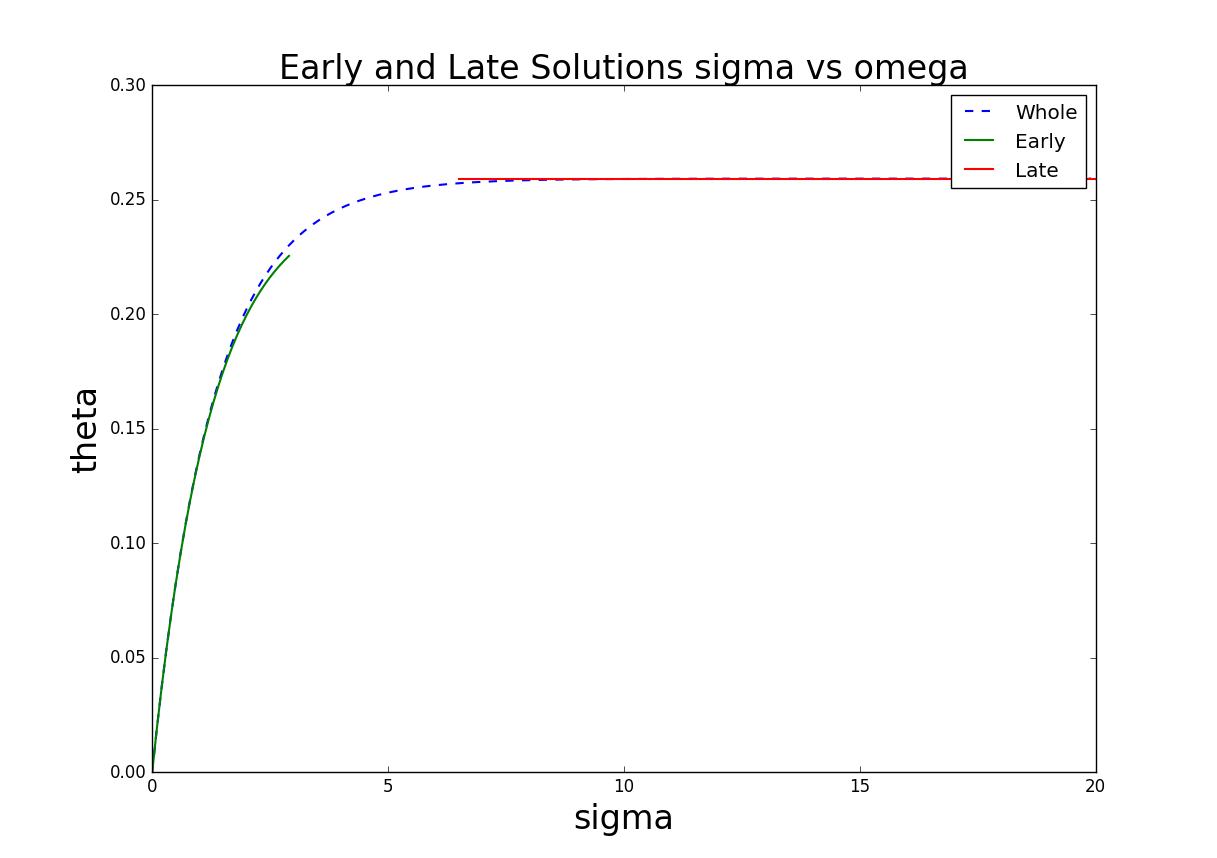
\includegraphics[width=\textwidth]{part1.png}
    \caption{Graph of the early solution, late solution, and RK4 solution}
\end{figure}
In this graph, $\sigma$ is proportional to time, and $\theta$ is proportional to energy and related to temperature. The fact that it has an asymptotic value for $\delta=0.2$ means that as much energy is being lost to the environment as is being generated in the chemical reaction. As time increases, the energy in the container approaches the asymptote. As the energy gets closer to the asymptotic value more and more energy is lost to the environment until the values become equal at
infinite time. One can also see that the short and long term solutions, shown as green and red lines, are accurate for large portions of the problem. With the numerical solution really only being necessary between 2.5 and 7.5.


\section*{Explosion Case ($\delta=1$)}
In the explosion case, delta is equal to 1 which is greater than delta critical. Since, delta is proportional to 1/h, this physically means that the amount of heat lost to the surrounding environment was small enough to allow the explosion to occur. Due to this, the temperature will increase asymptotically to infinity which would render our integration solver ineffective. In order to overcome this limitation, we reverse the the variables and invert the differential equation to get
$\frac{d\sigma}{d\theta}=\frac{1}{\delta e^{\theta}-\theta}$. Using fourth order Runge-Kutta to integrate the dimensionless differential equation, we found a numeric approximation of sigma in terms of theta with the initial condition $\sigma (0) = 0$. In order to determine the asymptotic value sigma explosion we used Simpson's method to approximate the integral from 0 to infinity of the differential equation. We found this value to be 1.3951 which matched the limit of sigma found in the numeric approximation. Using this value for sigma explosion, we were able to create a long term approximation for sigma valid for sufficiently large values of theta. We also used the same short term approximation as in the fizz case to approximate sigma for theta close to zero. 
\begin{figure}[H]
    \centering
    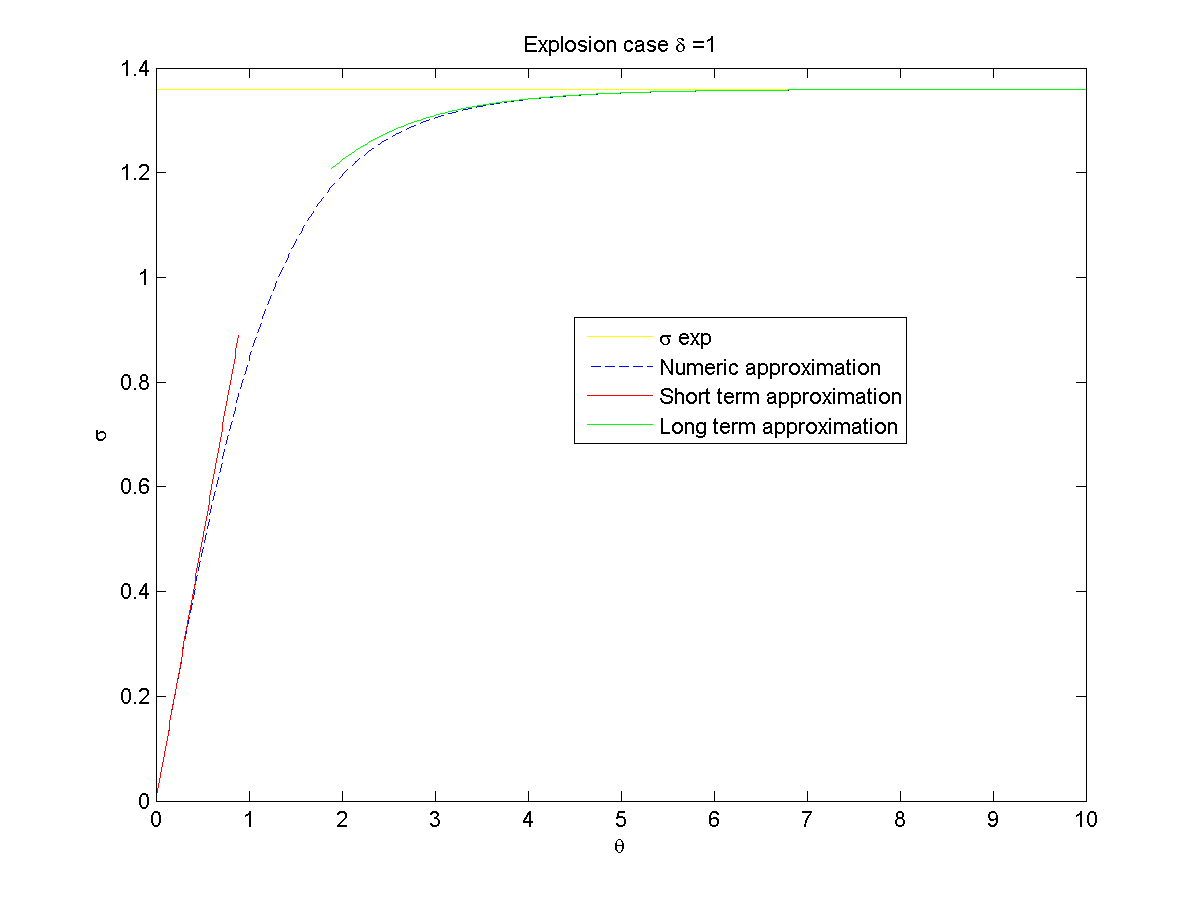
\includegraphics[width=\textwidth]{explosion.png}
    \caption{The graph of $\sigma$ and $\theta$ for the explosion case, showing that $\sigma$ asymptotes at $1.3951$}
\end{figure}
When theta approaches zero the differential equation approaches $\frac{1}{e^0-0}$ which is 1 so the short term solution is the line sigma = theta. When we plug in the dimensional variables we find that time and temperature are linearly related for time close to 0. When theta goes to infinity the differential equation goes to $\frac{1}{e^\theta}=0$. This means that as sigma (which is proportional to time) approaches the critical value of sigma explosion theta (proportional to temperature)
?blows up? to a very large value as the explosion happens and large amounts of heat generated by the reaction. As the system approaches the critical time, enough fuel has been burned up to sufficiently increase the energy of enough particles past the activation energy for the problem and the temperature increases exponentially as the energy used in activation the reaction is more than replaced by the energy given off in the reaction.
\section*{Conclusion}
We have analysed the non-adiabatic explosion problem in two separate instances using many numerical techniques, in one instance the heat was allowed to diffuse into the environment enough to cause the reaction to fizzle out and approach a limiting temperature. In the other instance, heat was retained sufficiently enough to allow the reaction to give off enough heat to cause an explosion. In both instances, similar asymptotic behavior was displayed, with the explosion  having a critical time
where temperature grew toward infinity and the fizzle having a critical temperature that was never surpassed as time grew to infinity. We learned the value that numerical methods have in modeling when analytic solutions are difficult or impossible to find.
\clearpage
\appendix
\section*{Appendix: Part 1}
Code for part 1, the fizzle case
\pythonexternal{fizzle.py}
\section*{Appendix: Part 2}
Helper functions for part 2, the explosion case\\
The function to be integrated:
\lstinputlisting{F.m}
Helper function to run Runge Kutta 4:
\lstinputlisting{RangeK.m}
Runga Kutta 4:
\lstinputlisting{RK4.m}
Simpson's Method:
\lstinputlisting{Simpson.m}
Short time solution function:
\lstinputlisting{ST.m}
Long time solution function:
\lstinputlisting{LT.m}
\end{document}
